\section{Séance 7 : Concurrence monopolistique, oligopole et comparaison des diverses formes de marché}






\subsection{Oligopole}
L'oligopole est l'un des 4 types de marché existants. C'est comme le marché du GSM. Trois ou quatre firmes, pas plus, c'est bloqué. Chaque firme se fait concurrence, mais avec une stratégie assez compliquée. On ne peut pas entrer sur le marché.


\subsection{Concurrence monopolistique}
La concurrence monopolistique est l'un des 4 types de marché existants. Elle est comme l'oligopole, mais on peut entrer dans le marché. Le terme \textit{concurrence} veut dire \textit{entrée possible}.

C'est le cas le plus connu ; les petits commerces. Il n'y a pas de substituts parfaits, ils ne sont pas tous au même endroit, etc.

Chaque épicerie a un petit pouvoir de monopole sur les maisons autour d'elle. Si le marché est très profitable, des gens en plus peuvent venir se greffer dessus et faire concurrence.

La concurrence monopolistique maximise son profit :
$$max( \Pi ) = RT - CT$$
$$\frac{d\Pi}{dQ} = RM - CM = 0 \Rightarrow RM = CM$$

\subsubsection{Court terme}
\begin{itemize}
	\item On a $RM - CM$
\end{itemize}

\subsubsection{Long terme}
\begin{itemize}
	\item Il y a les mouvements d'entrée ;
	\item Quand le marché est profitable, les firmes entrent ;
	\item Quand il n'est plus profitable, les firmes sortent ;
	\item Plus il y a de concurrents, moins on a de clients, car la concurrence est rude.
	\item Quand une firme entre, la profitabilité baisse car la demande est découpée, l'élasticité des consommateurs augmente (on a plus de substituts).
	\item Par contre, les coûts de production ne changent pas avec la concurrence. On les produit, c'est tout.
\end{itemize}

\subsection{Résumé des 4 types de marché}
En résumé, on a deux choses qui changent : le pouvoir de monopole, de nul à absolu, puis est-ce que l'entrée est possible ou pas. Le terme \textit{concurrence} veut dire \textit{entrée possible}.

La concurrence monopolistique par exemple veut dire qu'on a un petit pouvoir de monopole, on peut un peu augmenter
les prix, on offre une plus-value. La concurrence parfaite est quand on est tellement en concurrence qu'on ne peut pas toucher au prix.


%\begin{tabularx}{1.0\linewidth}{|*{5}{>{\centering\arraybackslash}X|}}

\newcolumntype{Y}{>{\centering\arraybackslash}X}
\begin{center}
\begin{tabularx}{1.0\linewidth}{@{}|l|Y|Y|Y|Y|@{}}

\hline
                                & Concurrence parfaite      & Concurrence monopolistique & Monopole & Oligopole\\\hline
Le profit de long terme est nul & \cellcolor{black!25} Vrai & \cellcolor{black!25} Vrai  &          &          \\\hline
$P = min(CMoT)$                 & \cellcolor{black!25} Vrai &                            &          &          \\\hline
$A l'optimum, CM=P$             & \cellcolor{black!25} Vrai &                            &          &          \\\hline

        
\end{tabularx}
\end{center}


\subsection{Comparaison des diverses formes de marché}



\subsubsection{Stratégies}


\begin{center}
	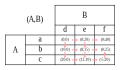
\includegraphics[height=4.5cm]{images/strategie.pdf}\\
	Tableau de stratégie
\end{center}
\begin{description}
	\item [A] possède trois stratégies différentes possibles (\textbf{a}, \textbf{b} et \textbf{c}) ;
	\item [B] possède trois stratégies différentes possibles (\textbf{d}, \textbf{e} et \textbf{f}) ;
	\item [A] n'a pas de stratégie dominante ;
	\item [B] a \textbf{f} comme stratégie dominante ;
	\item [(a,f)] et \textbf{(b,f)} sont les équilibres de nashs ;
\end{description}